
Un cristal bidimensional que ha despertado interés en la comunidad científica es el siliceno. 
De manera semejante al grafeno conformado por átomos de carbono, el siliceno también tendría una estructura 
hexagonal tipo panal de abeja conformada por átomos de silicio, por el hecho de encontrarse el silicio debajo 
del carbono en la tabla periódica y podría tener la hibridización de los orbitales 3s, $3p_{x}$ y $3p_{y}$ 
para conformar tres enlaces covalentes $sp^{2}$ -orbitales $\sigma$-, para formar la red hexagonal en el 
plano xy. \cite{arrieta2014sistemas}

\begin{figure}[H]
    \centering
    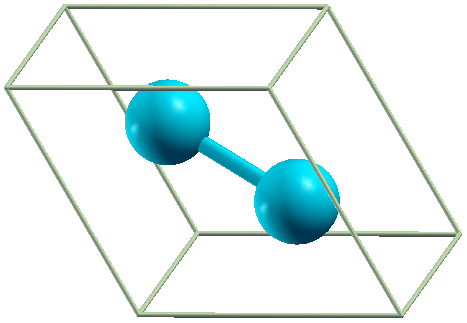
\includegraphics[scale=0.5]{images/silicene_cell.png}
    \caption{Estructura cristalina del Siliceno obtenida del archivo input con Xcrysden [Celda primitiva]}
\end{figure}

\begin{table}[H]
    \begin{center}
        \begin{tabular}{| c | c |}
            \hline
            \multicolumn{2}{ |c| }{\textbf{Archivo inicial}} \\ \hline
            ibrav & 4 \\ \hline
            nat & 2 \\ \hline
            ntype & 1 \\ \hline
            occupations & smearing \\ \hline
            degauss & 0.01 \\ \hline
            smearing & 'm-p' \\ \hline
            c & 12 \\ \hline 
            Atomic Positions Crystal & Si 0.33333333 0.66666667  0.491879248  \\
                                     & Si 0.66666667  0.33333333 0.533106764 \\  \hline
        \end{tabular}
        \caption{Principales paramétros del siliceno}
        \label{tab: Parametros del Siliceno}
    \end{center}
\end{table}

A continuación, realizaremos los siguientes cálculos y optimizaciones:

\begin{itemize}
    \item Optimización K-points [Siliceno]
    \item Optimización Lattice parameter (parámetro de red) [Siliceno]
    \item Cálculo de bandas [Siliceno]
    \item Densidad de estados sin considerar el spin [Siliceno] 
    \item Densidad de estados considerando el spin [Siliceno]
\end{itemize}

\vspace{0.5cm}

Veamos a continuación una representación del siliceno en su forma bidimensional.

\begin{figure}[H]
    \centering
    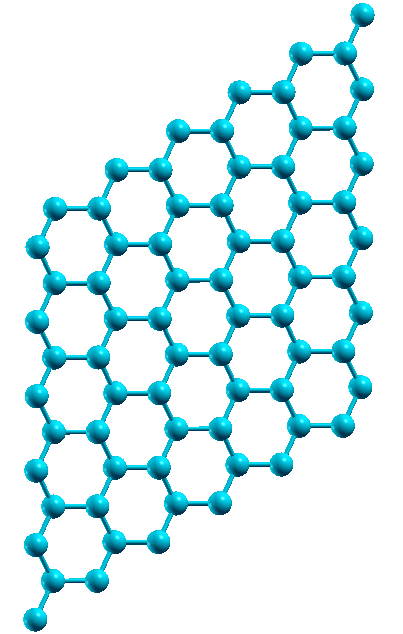
\includegraphics[scale=0.5]{images_siliceno/siliceno_2d.png}
    \caption{Estructura cristalina del Siliceno obtenida del archivo input con Xcrysden [Celda primitiva]}
\end{figure}

\newpage

% Optimización K-points [Siliceno]


\subsection{Optimización K-points [Siliceno]}

La primer optimización que realizaremos sobre el siliceno será la de puntos K. En nuestro archivo input estos
tienen la forma de la siguiente expresión: $ i \; i \; i \; 0 \; 0 \; 0$ donde $ i \in \mathbb{N}  $ .

\vspace{0.5cm}

Buscamos obtener un valor mínimo para i de tal manera que podamos observar una convergencia en la 
energía del sistema.

\begin{figure}[H]
    \centering
    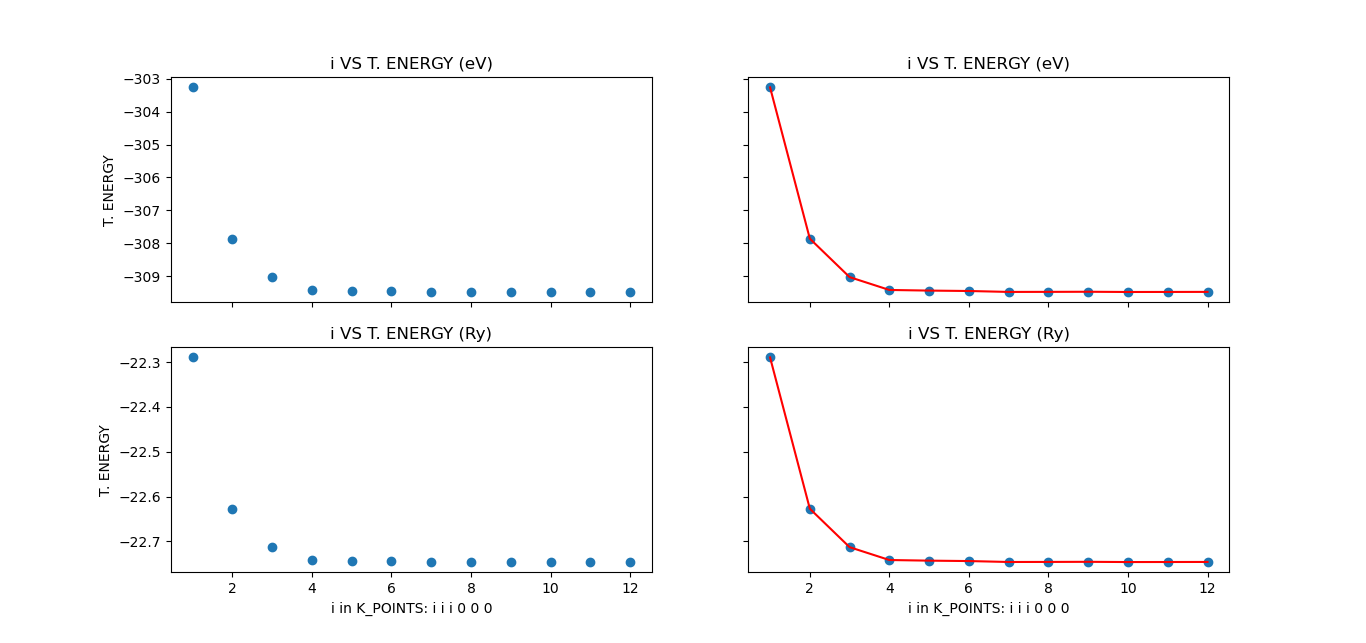
\includegraphics[scale=0.46]{images_siliceno/k_points_vs_t_energy_1_12.png}
    \caption{Gráfica que nos muestra la energía total del sistema contra la variación del parámetro k, nos centramos en el intervalo [1,12]}
\end{figure}

Vamos a analizar la misma gráfica en un rectangulo de inspección más pequeño.

\begin{figure}[H]
    \centering
    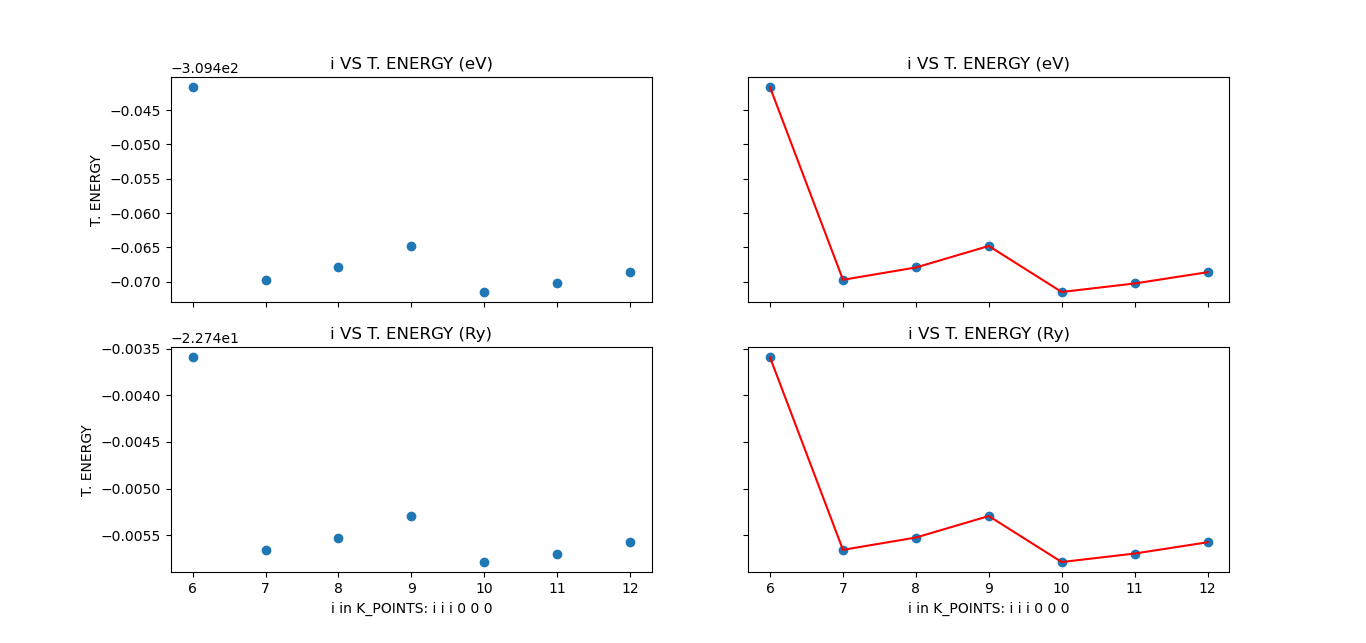
\includegraphics[scale=0.46]{images_siliceno/k_points_vs_t_energy_6_12.png}
    \caption{Gráfica que nos muestra la energía total del sistema contra la variación del parámetro k, nos centramos en el intervalo [6,12]}
\end{figure}

Observación: el valor de la variable dependiente (la energía total) empieza su convergencia cuando 
la variable independiente (i) empieza a tomar valores a partir de 7.


% Optimización Lattice parameter (parámetro de red) [Siliceno]


\subsection{Optimización Lattice parameter (parámetro de red) [Siliceno]}

Ahora vamos a buscar optimizar el valor del paramétro de red, haremos una inspección probando valores
en el siguiente intervalo [3.0, 4.5].
 
\vspace{0.5cm}

Buscamos obtener un valor mínimo para el paramétro de red de tal manera que podamos observar una convergencia 
en la energía del sistema.

\vspace{0.5cm}

Empezaremos desde el 3.0 y para cada uno haremos un calculo del tipo "relax", repetiremos el proceso
en saltos de 0.1 en 0.1 hasta alcanzar el valor de 4.5.

\begin{figure}[H]
    \centering
    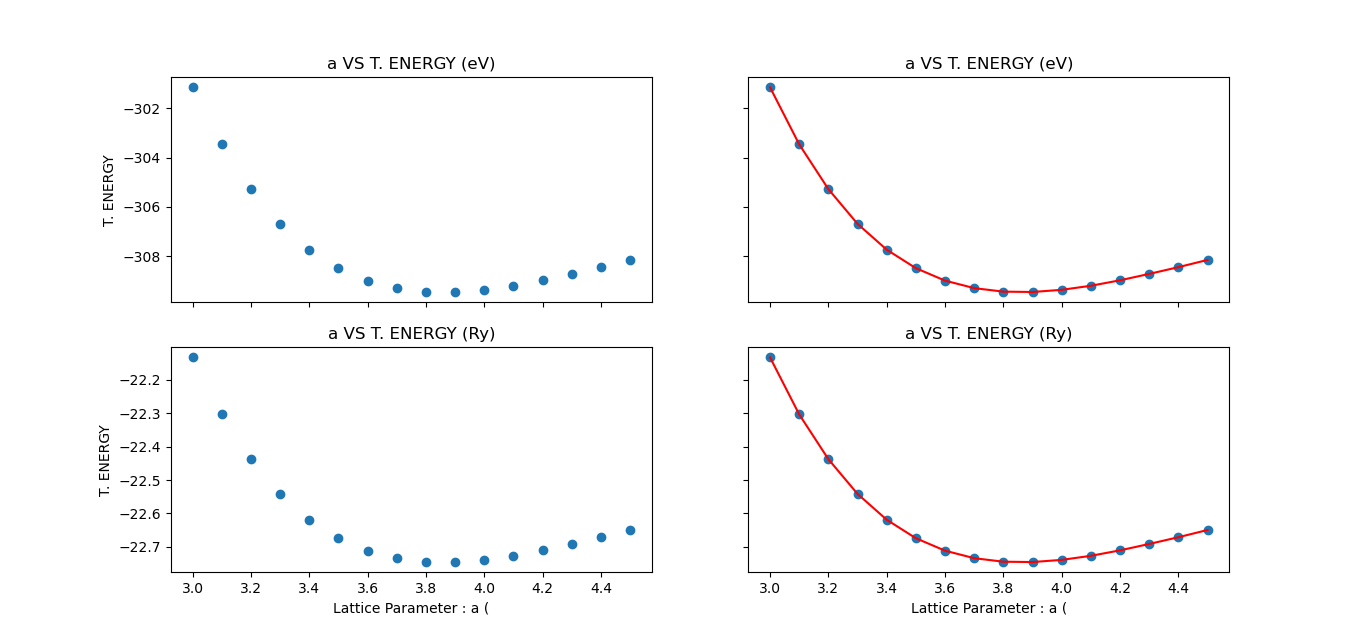
\includegraphics[scale=0.5]{images_siliceno/lattice_parameter_vs_T_energy.png}
    \caption{Gráfica que nos muestra la energía total del sistema contra la variación del parámetro k, nos centramos en el intervalo [3.0, 4.5]}
\end{figure}

Observación: el valor de la variable dependiente (la energía total) empieza su convergencia cuando 
la variable independiente (paramétro de red) empieza a tomar valores cercanos a 3.8.

\newpage

% Cálculo de bandas [Siliceno]

\subsection{Cálculo de bandas [Siliceno]}

En el siguiente apartado damos una gráfica con la estructura electrónica de bandas del siliceno. 
Para obtener esta estructura es necesario realizar la siguiente serie de cálculos.
Primero realizamos un cálculo con el módulo pw.x, después otro cálculo 
del tipo scf y por último uno del tipo bands.

Se llegó al siguiente gráfico:

\begin{figure}[H]
    \centering
    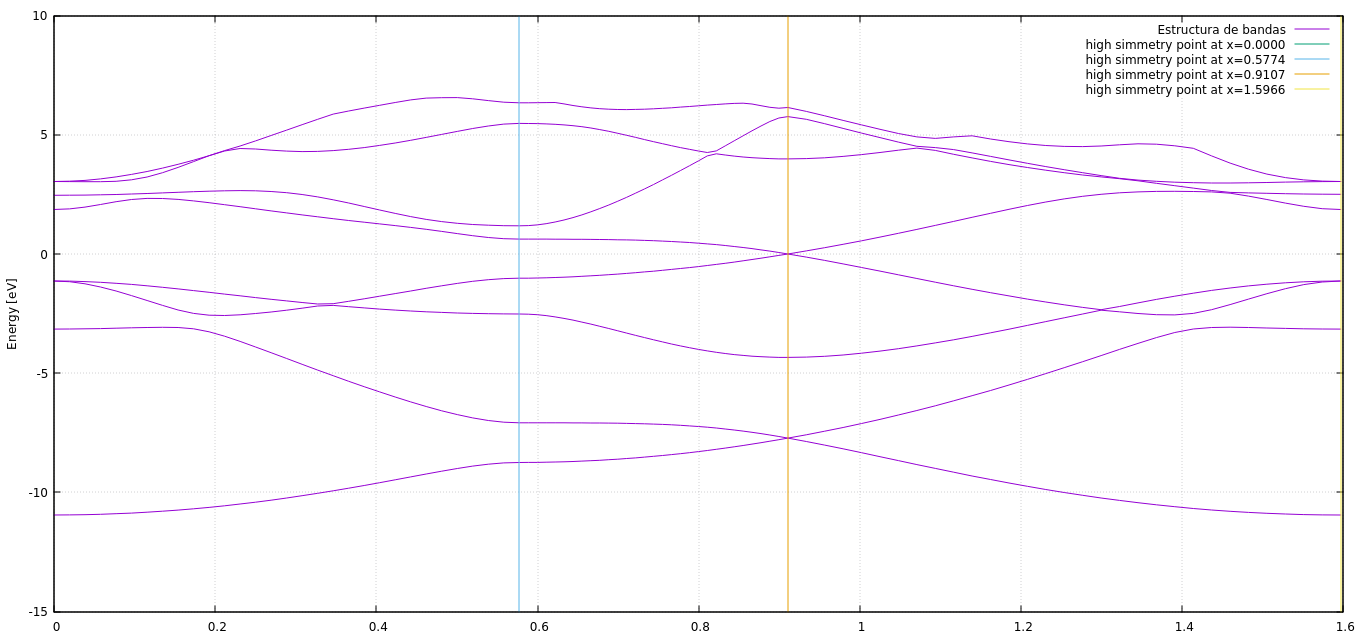
\includegraphics[scale=0.45]{images_siliceno/bands_structure.png}
    \caption{Gráfica que nos muestra la estructura de bandas del siliceno, cuyo cálculo fue elaborado por cuenta propia}
\end{figure}

En la literatura podemos encontrar estructuras similares, como por ejemplo:

\begin{figure}[H]
    \centering
    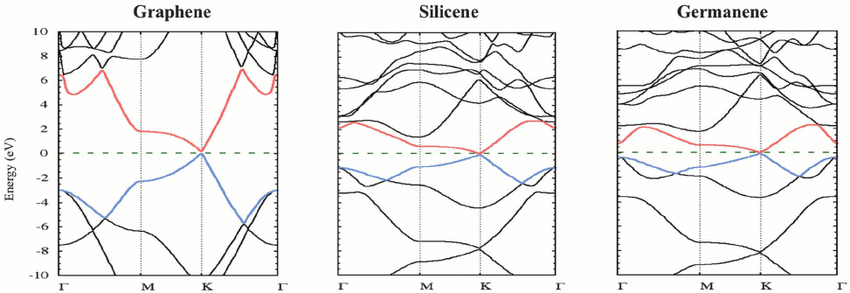
\includegraphics[scale=0.5]{images_siliceno/Band-structures-of-graphene-left-silicene-centre-and-germanene-right-Valence-and.png}
    \caption{Gráfica que nos muestra la estructura de bandas del siliceno (al centro) \cite{miro2014atlas} }
\end{figure}

Observación: Las estructuras propia y de la literatura muestran semejanza.

\newpage

% Densidad de estados sin considerar el spin [Siliceno]

\subsection{Densidad de estados sin considerar el spin [Siliceno]}

En el siguiente apartado damos una gráfica con la densidad de estados del siliceno. Para 
ello se hizo el cálculo dentro del mismo Quantum Espresso con el módulo pw.x, primero se hizo uno cálculo 
del tipo nscf y después otro del tipo DOS. También para este momento se trabajó con la estructura
ya relajada.

\vspace{0.5cm}

\textbf{Importante: En el siguiente cálculo no se consideró el spin.}

\vspace{0.5cm}

\begin{table}[H]
    \begin{center}
        \begin{tabular}{| c | c |}
            \hline
            \multicolumn{2}{ |c| }{\textbf{Parámetros destacados}} \\ \hline
            ecutwfc & 30 \\ \hline
            ecutrho & 240 \\ \hline
            occupations & smearing \\ \hline
            smearing & m-p \\ \hline
            degauss & 0.01 \\ \hline
            Parámetro de red & 3.88 \\ \hline
            nbnd & 8 \\ \hline
            k-points & 40 \; 40 \; 1 \; 0 \; 0 \; 0 \\ \hline
        \end{tabular}
        \caption{Algunos paramétros empleados en el siguiente cálculo.}
        \label{tab: Parametros del Siliceno sin spin}
    \end{center}
\end{table}

\vspace{0.5cm}

Se llegó al siguiente gráfico:

\begin{figure}[H]
    \centering
    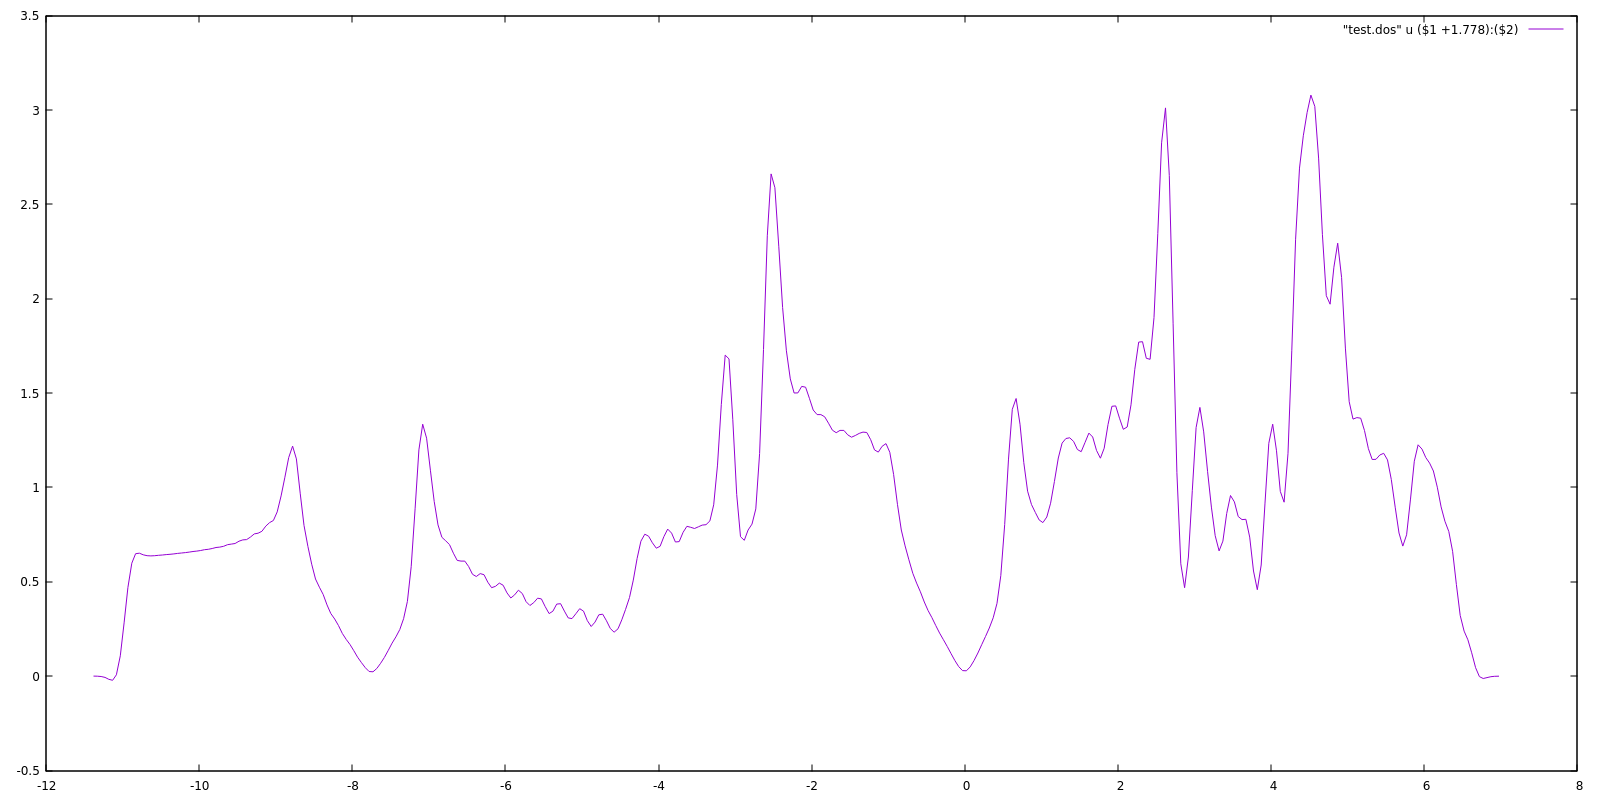
\includegraphics[scale=0.38]{images_siliceno/plot_sin_spin.png}
    \caption{Gráfica que nos muestra la densidad de estados del siliceno, sin considerar el spin.}
\end{figure}

% Densidad de estados considerando el spin [Siliceno]

\newpage

\subsection{Densidad de estados considerando el spin [Siliceno]}

En el siguiente apartado damos una gráfica con la densidad de estados del siliceno. Para 
ello se hizo el cálculo dentro del mismo Quantum Espresso con el módulo pw.x, primero se hizo uno cálculo 
del tipo nscf y después otro del tipo DOS.

\vspace{0.5cm}

\textbf{Importante: En el siguiente cálculo se consideró el spin.}

\vspace{0.5cm}

\begin{table}[H]
    \begin{center}
        \begin{tabular}{| c | c |}
            \hline
            \multicolumn{2}{ |c| }{\textbf{Parámetros destacados}} \\ \hline
            ecutwfc & 30 \\ \hline
            ecutrho & 240 \\ \hline
            occupations & smearing \\ \hline
            smearing & m-p \\ \hline
            degauss & 0.01 \\ \hline
            Parámetro de red & 3.88 \\ \hline
            nbnd & 8 \\ \hline
            k-points & 70 \; 70 \; 1 \; 0 \; 0 \; 0 \\ \hline
            nspin & 2 \\ \hline
            starting magnetization (1) & 1 \\ \hline
        \end{tabular}
        \caption{Algunos paramétros empleados en el siguiente cálculo.}
        \label{tab: Parametros del Siliceno con spin}
    \end{center}
\end{table}

\vspace{0.5cm}

Se llegó al siguiente gráfico:

\begin{figure}[H]
    \centering
    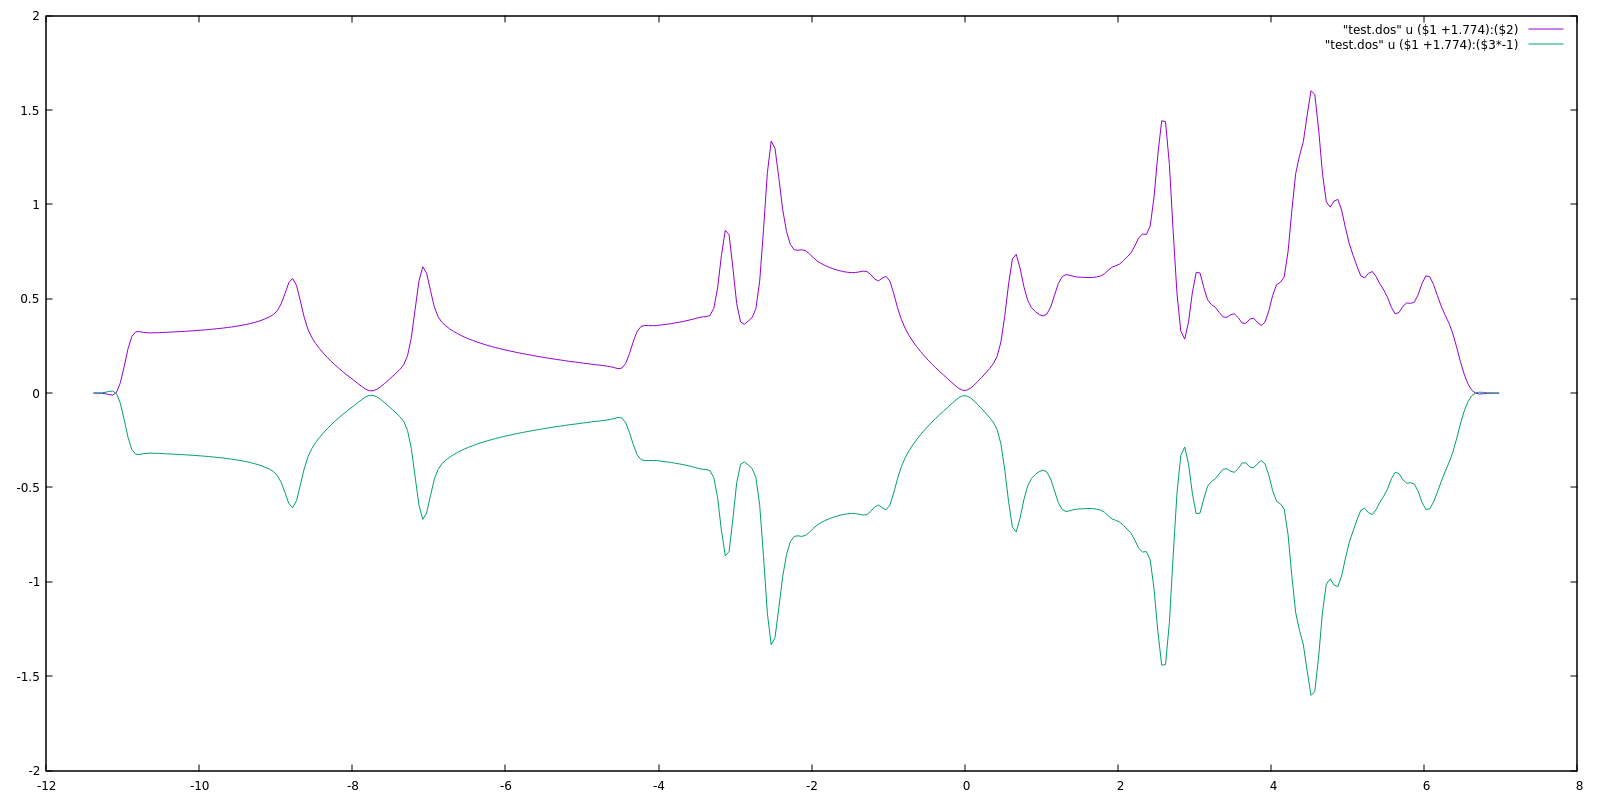
\includegraphics[scale=0.38]{images_siliceno/densidad_estados_con_spin.png}
    \caption{Gráfica que nos muestra la densidad de estados del siliceno, considerando el spin.}
\end{figure}

A continuación proporcionaremos una gráfica que nos muestra la energía por nivel orbital.

\begin{figure}[H]
    \centering
    \includegraphics[scale=0.38]{images_siliceno/silicio_energía_orbitales.png}
    \caption{Gráfica que nos muestra la energía en los orbitales del siliceno, considerando el spin.}
\end{figure}

\newpage